\documentclass[12pt,a4paper]{article}
\usepackage{pgf}
% \usepackage[condensed,math]{kurier}
% \usepackage[T1]{fontenc}
\usepackage{svg}
\usepackage{tikz}
\usepackage{stanli}
\usepackage{afterpage}
\usepackage{multirow}
\usepackage{subfig}
\usepackage{pgfpages}
\usepackage{svg}
\usepackage{rotating}

%\usepackage{times}


\pgfpagesdeclarelayout{boxed}
{
	\edef\pgfpageoptionborder{0pt}
}
{
	\pgfpagesphysicalpageoptions
	{%
		logical pages=1,%
	}
	\pgfpageslogicalpageoptions{1}
	{
		border code=\pgfsetlinewidth{2pt}\pgfstroke,%
		border shrink=\pgfpageoptionborder,%
		resized width=.9\pgfphysicalwidth,%
		resized height=.9\pgfphysicalheight,%
		center=\pgfpoint{.5\pgfphysicalwidth}{.5\pgfphysicalheight}%
	}%
}

\pgfpagesuselayout{boxed}


% Language setting
% Replace `english' with e.g. `spanish' to change the document language
\usepackage[english]{babel}

% Set page size and margins
% Replace `letterpaper' with `a4paper' for UK/EU standard size
\usepackage[a4paper,top=2cm,bottom=1.5cm,left=1.5cm,right=1.5cm,marginparwidth=1.75cm]{geometry}

% Useful packages
\usepackage{amsmath}
\usepackage{graphicx}
\usepackage[colorlinks=true, allcolors=blue]{hyperref}

\title{}
\author{}
\date{}

\begin{document}
	
	\newcommand{\subf}[2]{%
		{\small\begin{tabular}[t]{@{}c@{}}
				#1\\#2
		\end{tabular}}%
	}
	
	\begin{titlepage}
		\begin{center}
			\vspace*{3cm}
			
			\Huge
			\textbf{Features and concepts about progressive web applications}
			
			\vspace{0.8cm}
			\large
			
			\vspace{0.5cm}
			\LARGE
			
			
			\vspace{1.5cm}
			
			\textbf{}
            
\includegraphics[width=.6\textwidth]{utt.png}
			
			\vfill
			
			
			
			\vspace{0.8cm}
			
			
			
			\Large
			
			
			
			
		\end{center}
		\Large
		\begin{tabbing}
			\hspace*{1em}\= \hspace*{8em} \= \kill % set the tabbings
			\> Name:\>  \textbf{López Bautista Cristian Alexis} \\
			\> Group:\>  10-B \\
			\> Subject:\>  Progressive Web Applications  \\
			\> Professor:  \> Dr. Ray Brunet Parra Galaviz \\
			\> Date: \>  Wednesday, January 10th, 2024
		\end{tabbing}
		
	\end{titlepage}
	
	
	
	\section{Web applications}

    \paragraph{Modern web applications have very high user expectations now a days. The web applications are expected to be available round-the-clock from anywhere in the world, and usable from any device for any screen size. Security is must for end users’ data, should be flexible, and scalable to meet high demand occasionally. Additionally, it should have rich user experiences built on the client.
    It is hard to say for any application that it is good or bad. The web applications should have some characteristics which decides that the users will stick to that website for long or not. Following are few of the characteristics which the web application should have:
    }
    
    \subsection{Web applications characteristics}
    
    \subsubsection{Availability}

    \paragraph{Round the clock availability of the site is not an option. Even few seconds of site shutdown is a huge loss to the E-commerce websites. For these sites, the advantage of online sales is that they are available at any time and available to be accessible from any part of the world at. 
    }
    
    \subsubsection{Performance}

    \paragraph{A little extra time in page load for the user will make the user go away to other sites where the performance is better, and this results in revenue loss. You cannot afford the delay in presenting content to its visitors. Example, A one-second delay in loading your web pages is an 11\% drop in an e-commerce site’s page views and a 7\% drop in the conversion rate. Your website’s performance greatly impacts your business and can make all the difference during periods of heavy activity. 
    }
    
    \subsubsection{Scalability}

    \paragraph{You should have sufficient infrastructure to support your website and its visitors. A website should be able to scale to several visitors. At the same time the back-end servers, database, APIs, and services too should be able to scale. The amount of traffic they host can change by a factor of three or even more during periods of high activity such as sales during Thanksgiving.
    }
    
    \subsubsection{Security}

    \paragraph{Security is a very important factor to be considered to make sure that your website follows industry standards and guidelines. Some examples are password encryptions, using SSL encryption. Also, protecting personal data is a major concern for the end-users and your customers’ trust in your website’s security is more essential than ever. E-commerce sites are choice targets for hackers due to the immense value of the information that goes through them, such as credit card numbers. It is vital that you protect yourself and your customers.
    }
    
    \subsubsection{Functional}

    \paragraph{A website is created or designed to serve a purpose, maybe to address some specific area. Mixing the different types of functionalities on the website is not at all suggested. Example, you should not write a blog on an e-commerce website.
    }
    
    \subsubsection{Ease of use}

    \paragraph{A website should be easy to use with friendly and quick navigation to move around different pages on site. Quick navigation is always suggested for more useful pages or for the flow of pages.
    }
    
    \subsubsection{Content}

    \paragraph{Irrelevant content is not at all a good idea on any website. Users lose the interest the moment they come across any content which is not relevant for the website. For example, do not try to sell a car on a cooking blogging site.
    }
    
    \subsubsection{Modern}

    \paragraph{Using current trends and technologies always benefits. The website should be up to date with current trends and continuous changes in the technologies.
    }
    
    \subsubsection{Optimized}

    \paragraph{It is mandatory to optimize the website and its content for different devices, browsers, data speed, search engines, and users. If it is not done in the right way, users may leave your website. Example, If the website is not optimized for popular smartphones and their sizes, users may not want to visit your website after the first use.
    }
    
    \subsubsection{Responsive}

    \paragraph{Now a days, the application are built with the Mobile first concept. Responsive web design is a need for all websites now. A responsive website changes its layout and options to fit the device and browser size.
    }

    \section{Service-oriented web applications}

    \paragraph{A service-oriented application is an application that is composed largely of services, which are often in a hierarchy.}

    \begin{figure}[h!]
      \centering
      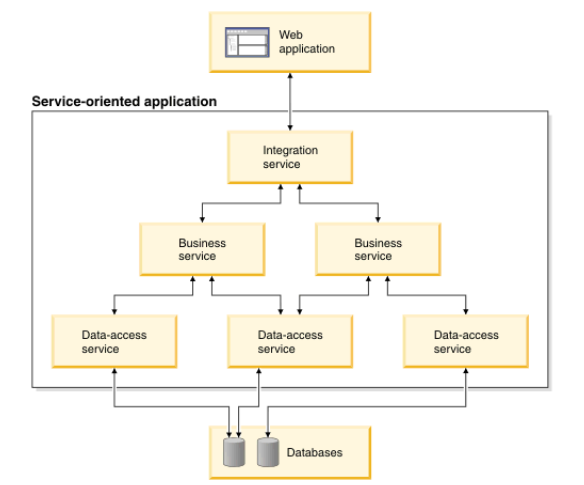
\includegraphics[width=0.5\textwidth]{diagrama.png}
      \caption{Service-oriented web applications diagram.}
    \end{figure}

    \paragraph{The topmost level contains one or more integration services, each of which controls a flow of activities, such as processing an applicant's request for insurance coverage. Each integration service invokes one or more business services.
    }

    \paragraph{The second level is composed of services that each fulfill a relatively low-level business task. The second business service calculates a quote and returns the quote to the software, such as a web application, that invoked the service-oriented application.
    }

    \paragraph{The third level consists of data-access services, each of which handles the relatively technical task of reading from and writing to data-storage areas, such as databases and message queues. A data-access service is most often invoked from the business layer, but the easy access of services allows for different uses. 
    }

   \subsection{Service-oriented web applications characteristics}

    \subsubsection{Web services are self-contained}

    \paragraph{On the client side, no additional software is required. A programming language with Extensible Markup Language (XML) and HTTP client support is enough to get you started. On the server side, a web server and a SOAP server are required. It is possible to enable an existing application for web services without writing a single line of code.
    }

    \subsubsection{Web services are self-describing}

    \paragraph{Neither the client nor the server knows or cares about anything besides the format and content of the request and response messages (loosely coupled application integration). The definition of the message format travels with the message; no external metadata repositories or code generation tool are required.
    }

    \subsubsection{Web services can be published, located, and invoked across the Internet}

    \paragraph{This technology uses established lightweight Internet standards such as HTTP and it leverages the existing infrastructure. Some other standards that are required include, SOAP, Web Services Description Language (WSDL), and UDDI.
    }

    \subsubsection{Web services are language-independent and interoperable}

    \paragraph{The client and server can be implemented in different environments. Existing code does not have to change in order to be web services-enabled.
    }

    \subsubsection{Web services are inherently open and standard-based}

    \paragraph{XML and HTTP are the major technical foundation for web services. A large part of the Web service technology has been built using open-source projects.
    }
    
    \subsubsection{Web services are dynamic}

    \paragraph{Dynamic e-business can become reality using web services because with UDDI and WSDL you can automate the web service description and discovery.
    }
    
    \subsubsection{Web services are composable}

    \paragraph{Simple web services can be aggregated to more complex ones, either using workflow techniques or by calling lower-layer web services from a web service implementation. Web services can be chained together to perform higher-level business functions. This chaining shortens development time and enables best-of-breed implementations.
    }
    
    \subsubsection{Web services are loosely coupled}

    \paragraph{Traditionally, application design has depended on tight interconnections at both ends. Web services require a simpler level of coordination that supports a more flexible reconfiguration for an integration of the services.
    }
    
    \subsubsection{Web services provide programmatic access}

    \paragraph{The approach provides no graphical user interface; it operates at the code level. Service consumers need to know the interfaces to web services, but do not need to know the implementation details of services.
    }
    
    \subsubsection{Web services provide the ability to wrap existing applications}

    \paragraph{Already existing stand-alone applications can easily integrate into the SOA by implementing a web service as an interface.
    }

    \section{Mobile applications}

    \subsection{Native apps}

    \paragraph{They are the most known apps due to their great advantages. Native mobile applications are those that are developed with a specific computer language, Xcode for iOS devices and Java (or Kotlin) for Android.}
    
    \paragraph{These types of mobile apps are found in marketplaces, like the App Store and Play Store, and from these platforms, you can download them for different devices, for example, for computers, tablets, or smartphones. }
    
    \paragraph{Native apps are highly recommended for companies because this type of application is the most secure type of app. Also, a lot of integrations and functionalities are available, and in this way, you can create the app that you want.}
    
    \paragraph{Although the time and costs of developing a native app are higher in comparison to other types of apps, you must consider that native mobile apps are developed for each operating system (iOS and Android), so the hours of work are much more. Also, it is important to say the high level of personalization and efficiency of native apps that provide the best user experience.}

    \subsection{Web apps}

    \paragraph{As their name says, these types of mobile apps are related to websites. Firstly, web apps are not developed for each operating system like native applications, but they are developed through JavaScript, CSS, and HTML-like website development. }
    
    \paragraph{This makes it possible for web apps can adapt to any system and device and they do not have to be downloaded. For these reasons, a responsive design is essential in these types of mobile applications. }
    
    \paragraph{Developing web apps is less expensive than native ones but also, they have worse efficiency, and generally, they need to be connected to the internet so that they work. Also, the level of personalization is less than in native apps.}
    
    \paragraph{As it is developed as a website and does not require a download, no approval from the app marketplaces is necessary either. In summary, this type of easy-to-develop application is a web page that looks like an app and is developed for projects with a lower budget.}

    \subsection{Hybrid apps}

    \paragraph{This category of mobile application, as its name suggests, is a mix of the previous two that we have talked about. Hybrid apps have features both native apps and web apps.}
    
    \paragraph{Hybrid applications are developed through JavaScript, HTML, and CSS as website development. However, with a hybrid app, you can access the functionalities and characteristics of the native apps.}
    
    \paragraph{This type of mobile application has its advantages and disadvantages too. On the one hand, it is not necessary to develop an app for each operating system. But on the other hand, you cannot access all the functionalities that a native app allows.}
    
    \paragraph{These tools are multiplatform and cheaper, so they tend to be adapted to projects that do not have enough resources to create a native app.}

    \section{Progressive web applications}

    \paragraph{A progressive web app (PWA) is a website that looks and behaves as if it is a mobile app. PWAs are built to take advantage of native mobile device features, without requiring the end user to visit an app store, make a purchase and download software locally. Instead, a PWA can be located with a search engine query and accessed immediately through a browser.}

    \paragraph{PWAs eliminate the need for e-commerce merchants to develop native apps for multiple mobile operating systems. Just like YouTube videos, PWA content is downloaded progressively, which provides the end user with a better user experience than a traditional website that uses responsive design. The term “progressive web apps” was coined in 2015 by designer Frances Berriman and Google Chrome engineer, Alex Russell.}

    \paragraph{The goal of PWAs is to blur the distinction between native apps and the mobile web by bringing most of the benefits of native mobile apps to the mobile browser. PWAs use standards-based technologies and run in a Container that is secure and accessible to anyone on the web. They can send web push notifications, work offline and be accessible from the home screen, just like a mobile app from an app store.}

    \subsection{Progressive web applications characteristics}

    \subsubsection{Responsiveness}

    \paragraph{Different companies produce gadgets with different screen sizes, and as a developer it's your responsibility to ensure all the different users enjoy the product regardless the device they are using. So, it's a good idea to make sure your app can be used on any screen size and its content is available at any view-port size.}

    \subsubsection{Installable}

    \paragraph{Research has shown that users tend to engage more with installed apps compared to visiting the official sites. Having a PWA as your product gives the users the look, feel and engagement of a normal app.}

    \subsubsection{Independent Connectivity}

    \paragraph{By keeping a user engaged to your app even while they are offline, provides a more consistent experience than dropping them back to a default offline page. A good example to illustrate this will be that of a music app, your users should be able to access offline playback and listen to saved music even without internet connection. Another good example is twitter app, a user is able to go back a read through tweets which they might have missed.
}

    \subsubsection{Discoverability}

    \paragraph{Since most PWAs are converted websites, it is fair to make them discoverable on the search engines, this will help generate extra traffic to your app. This also acts as an advantage over native apps which can't be discovered over the search engines.
}

    \subsubsection{Appearance}

    \paragraph{The appearance of the app should feel and look like that of a normal app, so be sure to include things like an app icon, this will help make it easily recognizable also things like splash screen will add the touch and feel of an app.
}

    \subsubsection{Cross Platform}

    \paragraph{PWAs are developed as web app first, which means that they need to work on all browsers/systems and not just a selected few. Users should be able to use them in any browser before they decide to install them.
}

\clearpage

	\section{Bibliography}

    \begin{enumerate}
    
      \item Fernández, C. (2023, October 13th). Types of mobile apps and their characteristics. ABAMobile. 
      
      \href{https://abamobile.com/web/types-of-mobile-apps-and-their-characteristics/ }{https://abamobile.com/web/types-of-mobile-apps-and-their-characteristics/ }
      
      \item IBM Corporation. (2022, June 16th). Service-oriented architecture (SOA). IBM Documentation.
      
      \href{https://www.ibm.com/docs/en/rbd/9.7?topic=overview-service-oriented-architecture-soa }{https://www.ibm.com/docs/en/rbd/9.7?topic=overview-service-oriented-architecture-soa }
      
      \item IBM Corporation. (2022, December 13th). Web services approach to a service-oriented architecture. IBM Documentation.
      
      \href{https://www.ibm.com/docs/en/was/9.0.5?topic=architecture-web-services-approach-service-oriented }{https://www.ibm.com/docs/en/was/9.0.5?topic=architecture-web-services-approach-service-oriented}
      
      \item Nyakundi, H. (2023, June 27th). What is a PWA? Progressive web apps for beginners. freeCodeCamp.org. 
      
      \href{https://www.freecodecamp.org/news/what-are-progressive-web-apps/}{https://www.freecodecamp.org/news/what-are-progressive-web-apps/}
      
      \item Sonavane, N. (2019, April 12th). Characteristics of a Web-Application. 
      
      \href{https://www.linkedin.com/pulse/characteristics-web-application-nripesh-sonavane/ }{https://www.linkedin.com/pulse/characteristics-web-application-nripesh-sonavane/ }
      
    \end{enumerate}
	
	
\end{document}